
%(BEGIN_QUESTION)
% Copyright 2007, Tony R. Kuphaldt, released under the Creative Commons Attribution License (v 1.0)
% This means you may do almost anything with this work of mine, so long as you give me proper credit

Switches, whether they be hand-actuated or actuated by a physical process, come in two varieties: {\it normally-open} (NO) and {\it normally-closed} (NC).  You are probably accustomed to seeing both types of switch represented in pushbutton form on schematic diagrams:

$$\includegraphics[width=15.5cm]{i02966x01.eps}$$

{\it Normally-open} pushbutton switches close (pass current) when actuated (pressed).  When un-actuated, they return to their ``normal'' (open) state.

{\it Normally-closed} pushbutton switches are just the opposite: they open (stop current) when actuated (pressed) and return to their ``normal'' (closed, passing current) state when un-actuated.

\vskip 10pt

This is simple enough to comprehend: the ``normal'' status of a momentary-contact pushbutton switch is the state it is in when no one is touching it.  When pressed, the pushbutton switch goes to the other (opposite) state.

Things get more confusing, though, when we examine {\it process switches}, such as pressure switches, level switches, temperature switches, and flow switches:

$$\includegraphics[width=15.5cm]{i02966x02.eps}$$

Define ``normal'' for each of these process switches.  In other words, explain what condition(s) each process switch must be in to ensure it is in the ``normal'' state; and conversely, what condition(s) need to be applied to each switch to force it into its other state.

\underbar{file i02966}
%(END_QUESTION)





%(BEGIN_ANSWER)

The ``normal'' condition for a process switch is the condition of {\it least stimulus}.  For example:

\vskip 10pt

\begin{itemize}
\item{} A pressure switch will be in its ``normal'' state when there is {\it minimum pressure applied}
\vskip 10pt
\item{} A level switch will be in its ``normal'' state when there is {\it no level detected by the switch}
\vskip 10pt
\item{} A temperature switch will be in its ``normal'' state when it is {\it cold}
\vskip 10pt
\item{} A flow switch will be in its ``normal'' state when there is {\it no flow detected by the switch}
\end{itemize}

%(END_ANSWER)





%(BEGIN_NOTES)

The ``normal'' status of an electrical switch, as universally defined by manufacturers, is a condition of:

\begin{itemize}
\item{} minimum stimulus
\item{} rest
\item{} a ``low'' sensing condition
\end{itemize}

Normally-Open (NO) contacts are sometimes called {\it form-A} contacts.

\vskip 10pt

Normally-Closed (NC) contacts are sometimes called {\it form-B} contacts.

\vskip 10pt

A switch having both NO and NC contacts is sometimes called {\it form-C}.



%INDEX% Switch, ``normal'' status

%(END_NOTES)


